\documentclass[12pt]{article}
\usepackage{amsmath}
\usepackage{graphicx}
\DeclareGraphicsExtensions{.pdf,.png,.jpg}

\newtheorem{theorem}{Theorem}[section]
\newtheorem{lemma}[theorem]{Lemma}
\newtheorem{definition}[theorem]{Definition}


\title{Small Time Optimality}
\date{}
\begin{document}
  \maketitle
  \section{Model}
	A Reed Shepp car model can be described by two variables $\boldsymbol{v}$ and $\boldsymbol{\omega}$ which are the speed and angular velocity. The turning radius is $r=\frac{ \boldsymbol{v} }{ \boldsymbol{\omega} }$. To simplify the model, $|\boldsymbol{v}|=1$, $|\boldsymbol{\omega}| \in [ \omega_{min}, \omega_{max}]$.\\
	
	We use $(x,y,\theta)$ to describe the state of a R.S car, $(x,y)$ being the position of the car, while $\theta$ being the orientation.
  
  \section{Optimal Path Upper Bound}
  %---------------------------------------------------------------------------
  % Theorem about the turning angle and min path length to turn such an angle.
  %---------------------------------------------------------------------------
  \begin{theorem}
  	There exist a minimium lenth $l$ for a R.S car to turn angle $\Delta\theta$. 
  \end{theorem}
  
  $\textbf{Proof}$: To turning a car with angle $\Delta\theta$ with the least amount of time, The control has to be $l^{+}l^{-}l^{+}l^{-}l^{+}...$ or $r^{+}r^{-}r^{+}r^{-}r^{+}...$ (keep turning counterclockwisely or clockwisely), with the max angular velocity. Therefore the turning radius is $r_{min}=\frac{ |\boldsymbol{v}| }{\omega_{max} }$.\\ 
  
  Assume the $i$-th operation turns $\Delta\theta_{i}$ angles, the number of operations is $n$ ($\forall{\Delta\theta_{i}} \geq 0$ or $\forall{\Delta\theta_{i}} \leq 0$, and $\sum_{i=1}^{n}\Delta\theta_{i} = \Delta\theta$). The total path length of these operation is:\\
  
  $l = \sum_{i=1}^{n}r_{min}\Delta\theta_{i}$ = $r_{min}\sum_{i=1}^{n}\Delta\theta_{i}$ = $r_{min}\Delta\theta$.

  which has nothing to do with the number of operations, neither with the angle of each turn.  
  
  %---------------------------------------------------------------------------
  % Theorem about the upper bound of a path being optimal.
  %---------------------------------------------------------------------------
  \begin{theorem}
  	For a start configuration s = $(x_{s},y_{s},\theta_{s})$, a goal configuration g = $(x_{g},y_{g},\theta_{g})$ and a path $\sigma$ with length $l$. $\sigma$ cannot be the optimal path if $l > r_{min}\pi + |SG|$, where S and G are $(x_{s}, y_{s})$ and $(x_{g}, y_{g})$.
  \end{theorem} 
  
  $\textbf{Proof}$: Consider steering a R.S car with small-time controlability using $l^{+}l^{-}l^{+}l^{-}l^{+}...$ or $r^{+}r^{-}r^{+}r^{-}r^{+}...$ operations. when the number of operation keeps increasing, the position offset decreases(limit to 0). A naive way of moving the car is to 1. steer the car from start orientation to $\vec{SG}$ direction, 2. move the car from S to G, 3. steer the car from $\vec{SG}$ direction to goal orientation.\\
  
  It can be proved that 1 and 3 steps can steer the car with a maxinum angle of $\pi$. ( list all kinds of possible orientations then it can be shown. I omit it here. )\\
  
  Thus the path length of this strategy is $L = \frac{\pi\boldsymbol{v}}{\boldsymbol{\omega}} + |SG| \geq r_{min}\pi + |SG|$\\
  
  If a path planning algorithm gives a path $\sigma$ with length $ l > r_{min}\pi + |SG|$, then the naive strategy is even better. $\sigma$ is clearly not the optimal path.\\
   
  %---------------------------------------------------------------------------
  % Theorem about the small time optimality.
  %---------------------------------------------------------------------------
  \begin{theorem}
  	If there is clearance of size $R > \frac{r_{min}•\pi}{2}$ at any point p in workspace, there exist a $R_{in}$-ball centered at p, $R_{in} \in (0, R)$, such between any points in the $R_{in}$-ball with any orientaion, there exists a feasible optimal trajectory.
  \end{theorem} 
  
  $\textbf{Proof}$: Assume $S = (x_{s}, y_{s})$ and $G = (x_{g}, y_{g})$ with orientations $\theta_{s}$ and $\theta_{g}$ are start and goal positions in workspace. We denode $|SG| = 2\delta$. \\
  
  With Theorem 2.2, we know that the optimal path $\sigma$ must satisfy the property of lenth $l <= r_{min}\pi + 2\delta$. Assume $C$ being a point in the workspae and $|SC|+|GC| \leq r_{min}\pi + 2\delta$. C is in an ellipse with foci's S and G. \\ 
  
  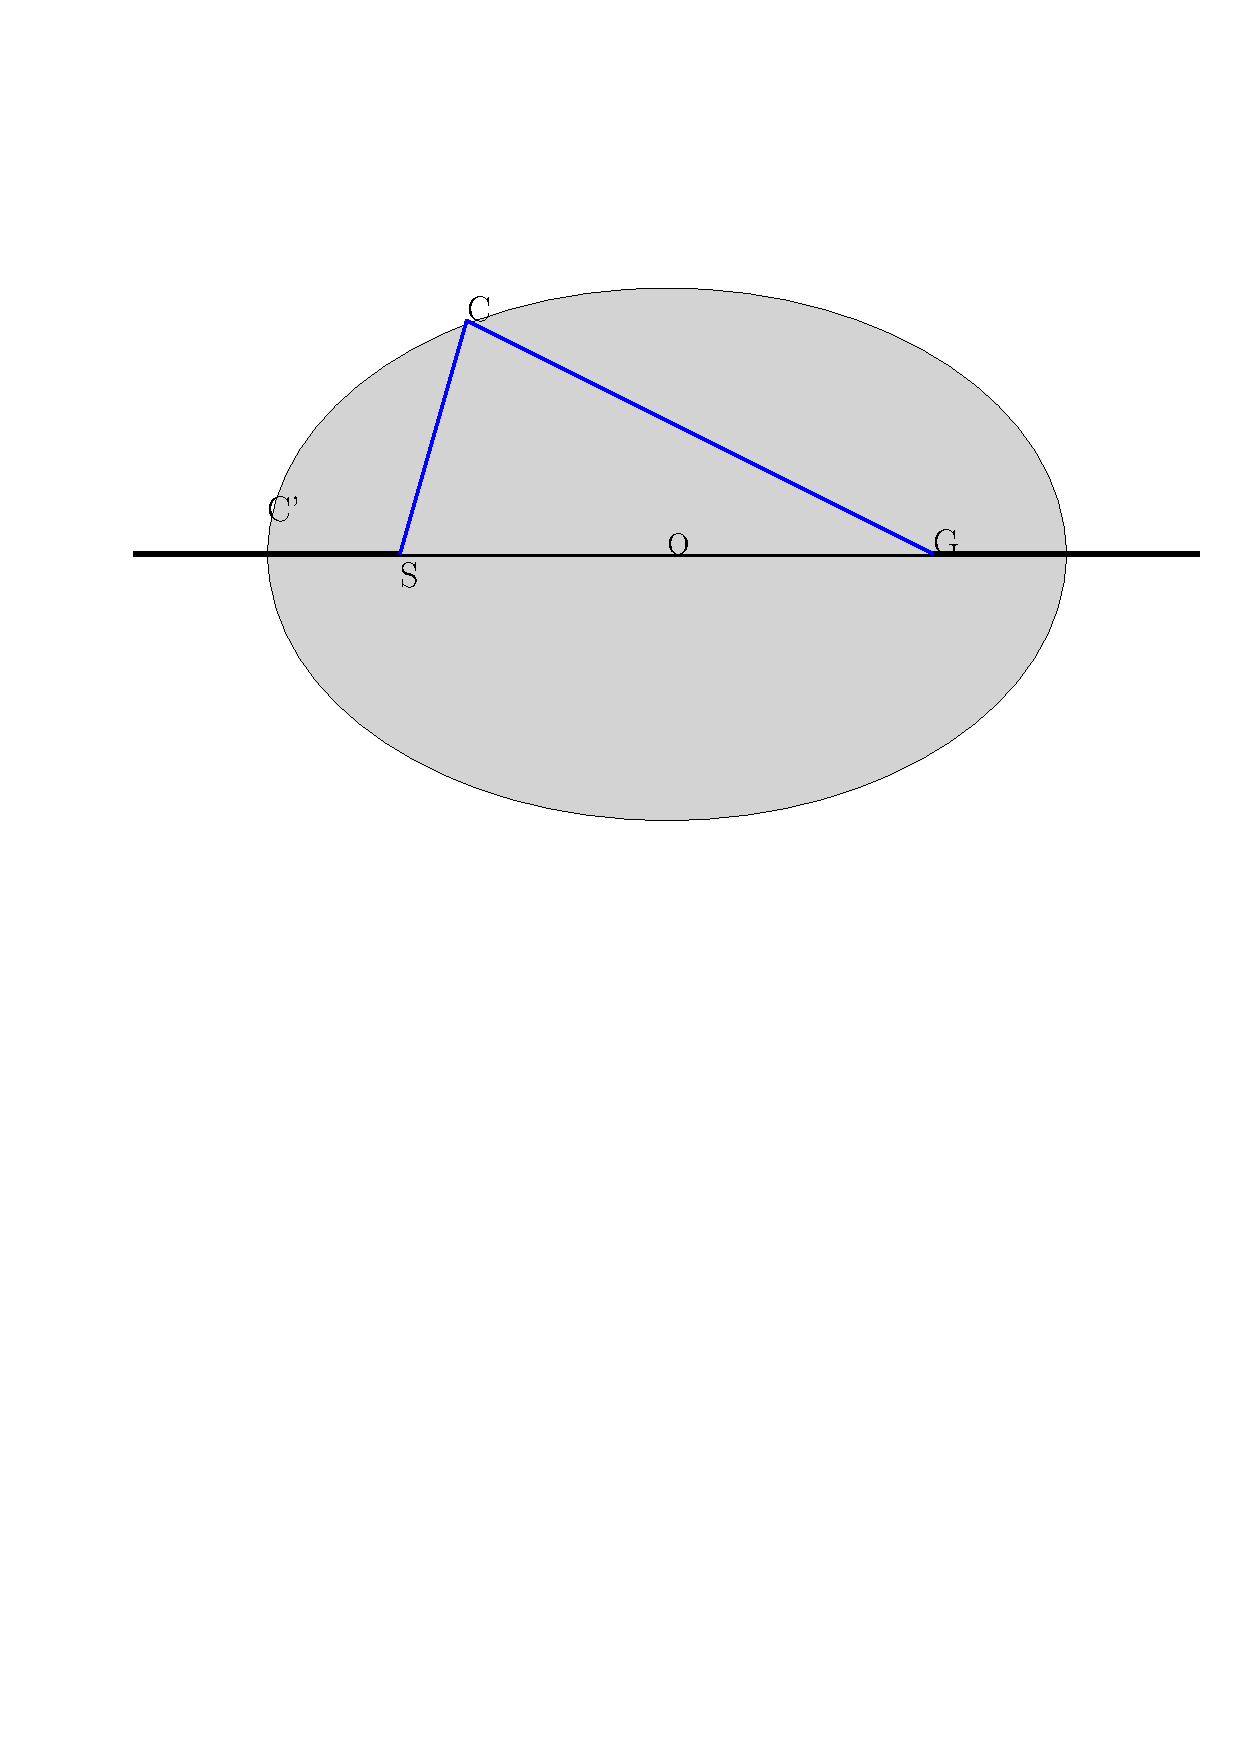
\includegraphics[scale=0.7]{Ellipse}\\
  
  Since any point P out side the ellipse will have $|SP| + |PG| > r_{min}\pi + 2\delta$, the optimal path from S to G with any orientation must be within the ellipse.\\
  
  $C'$ is a intersect point of line $SG$ and the ellipse. $O$ is the mid point of S and G. \\
  
  $\Longrightarrow$ $|SO| = |OG| = \delta$. $|C'S| + |C'G| = r_{min}\pi + 2\delta = 2|C'S| + |SG|$
  
  $\Longrightarrow$ $|C'S| = \frac{r_{min}\pi}{2}$\\
  
  By rotating S and G about their mid point O, the trajectory of C' is the edge if another ball with radius $\delta + \frac{r_{min}\pi}{2}$. And between any points in the inner ball, there must exist an optimal trajectory without leaving the outter ball. \\
  
  This two balls have radius difference of $\frac{r_{min}•\pi}{2}$.
  
\end{document}